\documentclass{sasbase}

\usepackage{lipsum}
\usepackage{enumitem}
\usepackage{graphicx}

\begin{document}

\title{Informationsblatt der APB}
\place{Ludwigsburg}
\datum{13. November 2017}
\edition{1}

\setcounter{secnumdepth}{5}

\mytitle

% OPTIONAL
%\squarestyle
% OR
\parensstyle

\section{Politische Bildung}
Das Bundesgesetzblatt beinhaltet auch immer FAQs zu neuen Gesetzen und der Funktionsweise der staatlichen Organe.
Fragen k\"{o}nnen gerne jederzeit an den Ausschuss f\"{u}r politische Bildung gesendet werden, diese werden so fr\"{u}h als m\"{o}gliche bearbeitet und in der n\"{a}chsten Ausgabe beantwortet.

\topic{Verfassung}
\begin{question}{Wie ist Goethopia aufgebaut?}
	Wie in jeder Demokratie ist das Grundger\"{u}st Goethopias das Volk. Anders als in manchen L\"{a}ndern ist in Goethopia absolut jeder wahlberechtigt, es gibt keine Altersgrenze. Die B\"{u}rger w\"{a}hlen in einer demokratischen Wahl Parteien, welche deren Interessen im Parlament vertreten. Welches Parteimitglied dann wirklich in das Parlament einzieht, ergibt sich \"{u}ber die Sitzeverteilung. Hier ein Beispiel zur Sitzverteilung im Parlament nach der Wahl:
	\begin{center}
		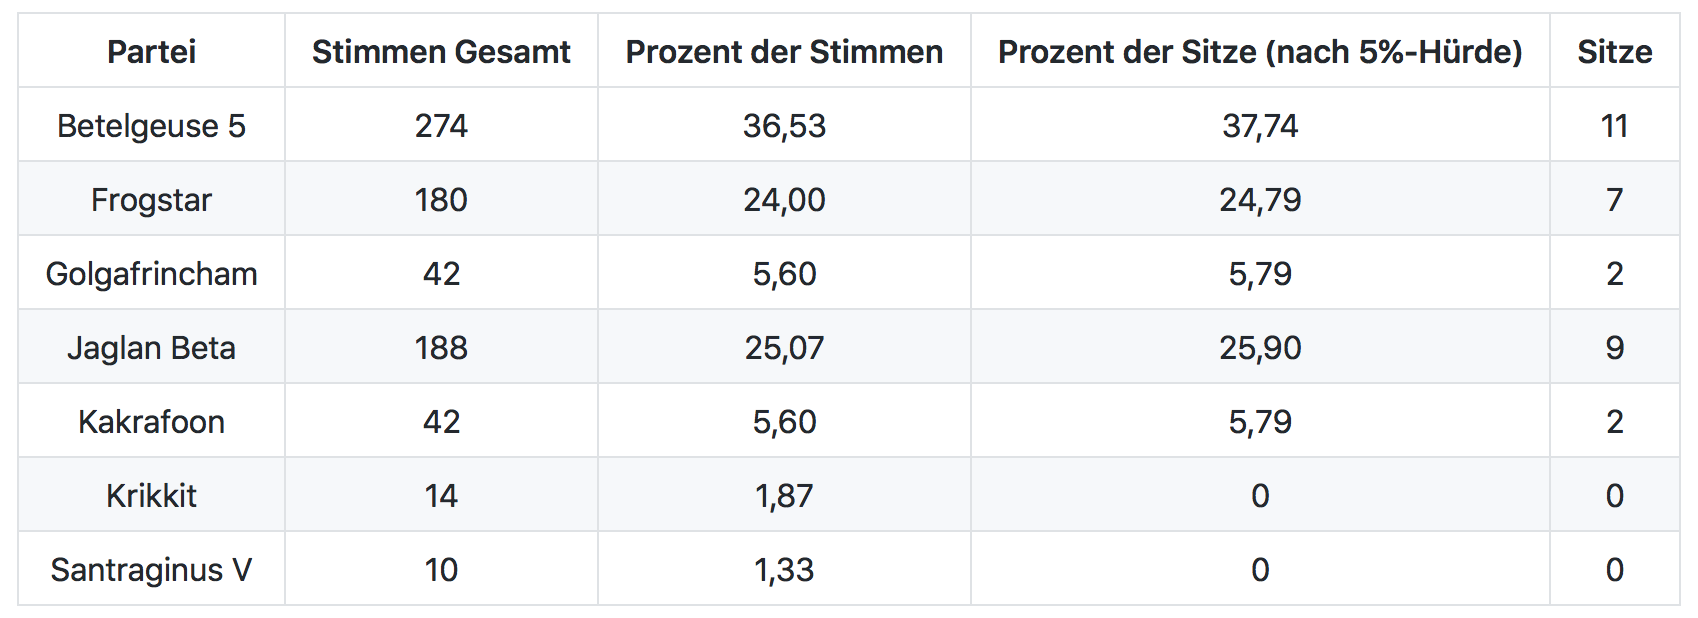
\includegraphics[width=8cm]{Tabelle_Beispiel_Sitzverteilung.png}
	\end{center}
	Hieraus ergibt sich nun folgende Sitzverteilung:
	\begin{center}
	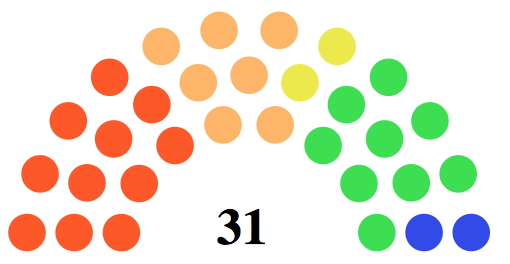
\includegraphics[width=8cm]{Parlament.png}
	\end{center}
Es ist nun am Parlament, eine Parlamentspr\"{a}sidentin zu bestimmen und eine mehrheitsf\"{a}hige Regierungskoalition zu bilden. In diesem Fall sind 16 Sitze ben\"{o}tigt, denkbar w\"{a}ren also folgende Koalitionen:
	\begin{enumerate}[label=-]
		\item \textbf{Betelgeuse 5}, Jaglan Beta (20 Sitze)
		\item \textbf{Betelgeuse 5}, Frogstar (18 Sitze)
		\item \textbf{Jaglan Beta}, Frogstar (16 Sitze)
	\end{enumerate}
	Das Parlament w\"{a}hlt nun eine Kanzlerin, welche wiederum ihr Kabinett, bestehend aus den Ministerien, ernennt. Zu den weiteren Aufgaben des Parlamentes geh\"{o}rt die Gesetzeserlassung und Wahl der Richter.
	\begin{center}
	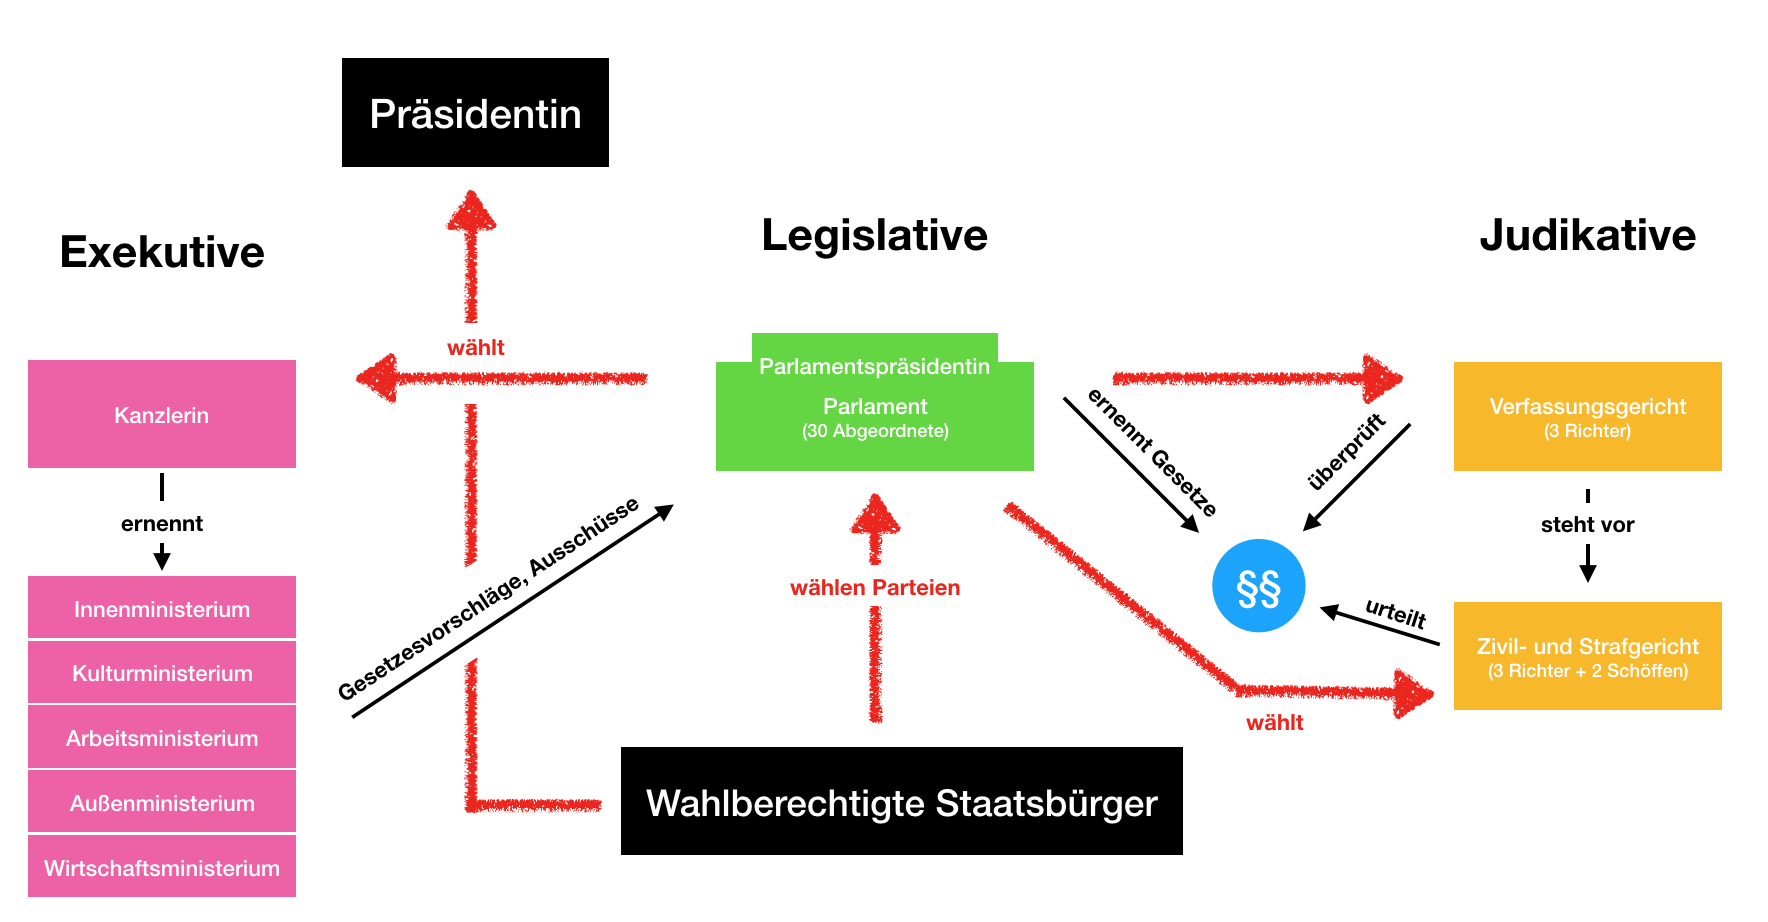
\includegraphics[width=8cm]{Verfassung.png}
\end{center}
\end{question}

\topic{Wahl}
\begin{question}{Wann wird die Wahl stattfinden?}
	Das Datum f\"{u}r die Wahl ist noch nicht festgelegt, voraussichtlich zwischen Weihnachtsferien und Osterferien. Sie werden auf jeden Fall dar\"{u}ber informiert, wenn der Wahltermin beschlossen wurde.
\end{question}
\begin{question}{Wie gr\"{u}nde ich eine Partei?}
	Damit eine Partei bei der Wahl zugelassen werden kann, muss sie mindestens \"{u}ber 10 Parteimitglieder und 20 Unterschriften verf\"{u}gen (siehe Artikel \ref{Wahlrecht}). Dies soll verhindern, dass es zu einer Flut von Parteigr\"{u}ndungen kommt. Wir empfehlen folgende Schritte, um erfolgreich bei der Wahl zugelassen zu werden:
	\begin{enumerate}
		\item \textbf{Festlegen der Parteigrunds\"{a}tze:}\\ Dieser Schritt ist notwendig, damit andere B\"{u}rgerinnen sich dazu entschlie{\ss}en k\"{o}nnen, der Partei beizutreten. Hier geht es nicht um ein konktretes Parteiprogramm, sondern um das Abstecken der Prinzipien, denen sich die Partei verordnet f\"{u}hlt.
		\item \textbf{Parteimitglieder anwerben:}\\ Es ist wichtig, dass gerade junge Parteien schnell wachsen und sich Mitstreiter finden, die gemeinsam die Partei vorantreiben. Erst wenn man die gesetzliche Mindestgr\"{o}{\ss}e erreicht hat, empfiehlt es sich, sich detailliert mit Inhalten auseinanderzusetzen.
		\item \textbf{Parteiprogramm erstellen:}\\ Hierf\"{u}r ist es sinnvoll, wichtige Kernpunkte aufzuteilen, sodass jedes Mitglied sich einen kleinen Teil des Parteiprogramms \"{u}berlegt. Danach sollte das Parteiprogramm beschlossen werden.
		\item \textbf{Kandidatenliste festlegen:}\\ Die Kandidatenliste bestimmt, wer ins Parlament einzieht. Erh\"{a}lt eine Partei 10 Sitze, so erhalten die ersten 10 Pl\"{a}tze auf der Parteiliste einen Sitz im Parlament.
		\item \textbf{Partei zur Wahl anmelden:}\\ Daf\"{u}r gen\"{u}gt es, Parteiname, Liste und Unterschriften/Mitglieder einfach an den Ausschuss f\"{u}r politische Bildung weiterzureichen.
		\item \textbf{Wahlwerbung machen:}\\ Dies ist der letzte Schritt. Nun gilt es, sich als Partei den B\"{u}rgerinnen \"{u}berzeugend zu pr\"{a}sentieren!
	\end{enumerate}
\end{question}

\begin{question}{Wie wird man Pr\"{a}sidentin?}
	Um Pr\"{a}sidentin zu werden, muss man Unterschriften von 10 B\"{u}rgern vorweisen und am 01.06.2018 mindestens 12 Jahre alt sein (siehe Artikel \ref{Präsidentin}). Wenn beide Bedingungen erf\"{u}llt sind, reicht es, sich mit Nachweis beim Ausschuss f\"{u}r politische Bildung offiziell zu bewerben. Danach empfiehlt es sich, weiterhin Wahlwerbung zu betreiben.
\end{question}

\section{Impressum}
Agentur f\"{u}r politische Bildung, stellvertretend Christian Merten und Nils Hebach.
\end{document}
